\section{Results and Analysis}

\subsection{The Arrow}
	\label{sec:arrow}
We chose to use a paper airplane model called ``The Arrow" to conduct the experiments. See Figure~\ref{fig:arrow} for a picture of The Arrow. We chose this model because it is easy to construct and rigid in structure. Due to its relatively small wing aspect ratio, The Arrow experiences little flapping motion; as a result, its flight better resembles what is assumed in theory. We constructed three The Arrow paper airplanes in order to reduce any model-specific measurement error. See Figure~\ref{fig:arrowdimension} for the weight and dimensions of these three airplanes. 

\begin{figure}[hl]
  \centering
    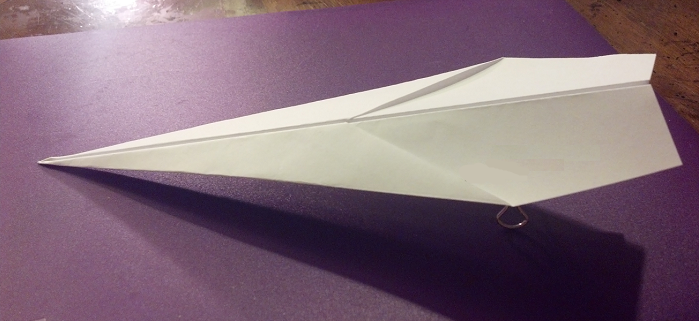
\includegraphics[scale=0.6]{figures/arrow.png}
    \caption{A picture of The Arrow. It is one of the most common paper airplane models. It has a long flight range and is easy to construct.}
  \label{fig:arrow}
\end{figure}

\begin{figure}[hl]
  \centering
    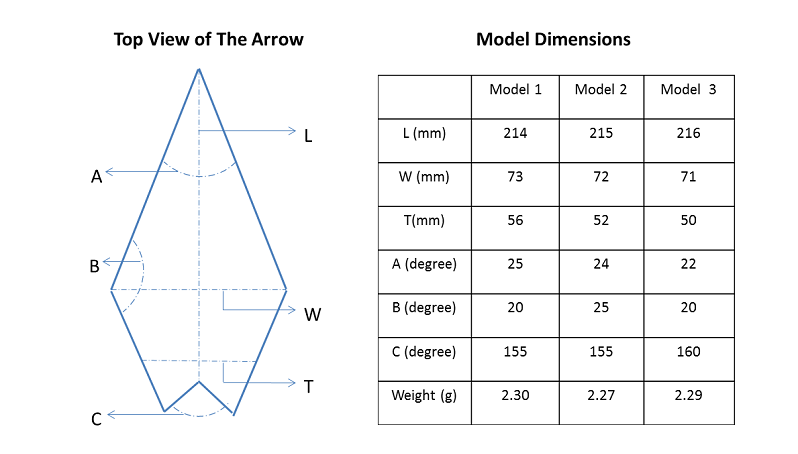
\includegraphics[scale=0.4]{figures/arrowdimension.png}
    \caption{Weight and dimension of the three paper airplanes.}
  \label{fig:arrowdimension}
\end{figure}

We launched the paper airplanes manually, and developed an iPhone application to record the launching acceleration and time (see appendix for the source code). A perosn was trained to launch these airplanes with consistency: the paper airplane started right above the launcher's shoulder and was released when the launcher's arm was fully extended. The launching height was measured to be 146cm and the launching distance was measured to be 60cm. The acceleration during the launch was measured to be 3g. Using these numbers we found the releasing speed of the paper airplanes to be 6m/s. 

\subsection{Stability vs Center of Gravity}
\label{sec:centergravity}
We attached a 2.9 gram paper clip to various positions of the paper airplanes. The paper clip weighed similar to the paper airplanes(see Figure~\ref{fig:arrowdimension} for the airplanes' weight), and its location effectively shifted the center of gravity of the paper ariplanes (see Figure~\ref{fig:clip}).

\begin{figure}[hl]
	\centering
		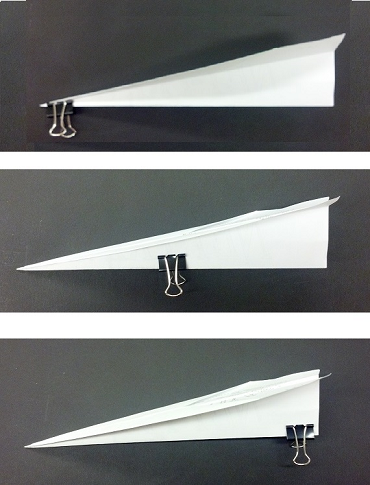
\includegraphics[scale=0.6]{figures/clip.png}
		\caption{We attached a 2.9 gram paper clip to various positions on the paper airplane to shift its center of gravity.}
	\label{fig:clip}
\end{figure}

We then launched the paper airplanes in the manner described in section~\ref{sec:arrow}. To reduce measurement noise, we performed ten launches for each of the paper airplanes at each of the center of gravity settings (a total of 90 launches). To measure flight stability, we recorded the number of x, y, and z-rotations the paper airplane had completed during its flight. See Figure~\ref{fig:rotation} for a classification of these rotations. 

\begin{figure}[hl]
	\centering
		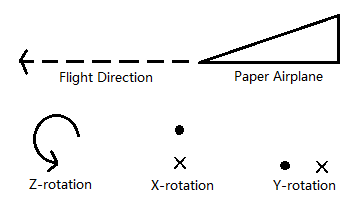
\includegraphics[scale=1]{figures/rotation.png}
		\caption{A schematic illustrating different types of rotation during flight.}
	\label{fig:rotation}
\end{figure}

We also measured the distance traveled when the paper airplane landed. A stable flight should have very few rotations and consistent distance traveled. Figure~\ref{fig:centerofgravity} shows the result. 

\begin{figure}[hl]
	\centering
		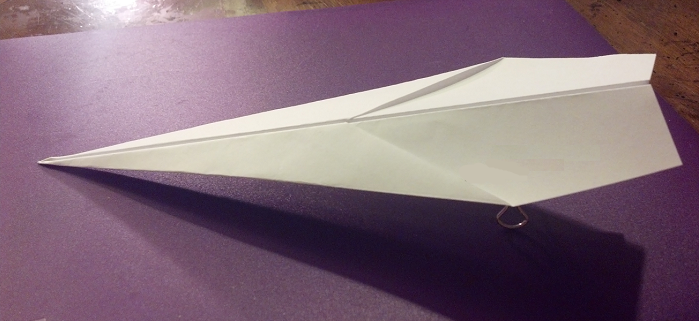
\includegraphics[scale=0.5]{figures/centerofgravity.png}
		\caption{Flight stability vs the center of gravity. Flight distance standard deviation and number of rotations in the air provide qualitative measures of stability: the smaller the standard deviation and fewer the number of rotation, the more stable the flight. We shifted the flight's center of gravity by attaching a metal clip to various positions on the paper airplane.}
	\label{fig:centerofgravity}
\end{figure}

When the clip was attached at the rear of the paper airplane, we observed both y and z-rotations. The flight was extremely turbulent and the paper airplane lost direction soon after launch. As a result, the distance traveled was short. When the clip was attached to the front or the middle of the paper airplane, no rotation was observed during flight. To compare the stability, we looked at the standard deviation of distance. When the clip was attached to the front, the standard deviation was smaller, indicating more consistent and stable flights. In conclusion, we found that the stability of flight decreases as the center of gravity shifts towards the rear of the airplane. This supports our analysis in section~\ref{sec:long_stability}. One interesting thing to notice is that when the clip was attached to the middle of the paper airplane, the distance traveled was the longest. This suggests there's a possible trade-off between stability and lift coefficient. 


\subsection{Stability vs Wing Angles}
As discussed in section~\ref{sec:dihedral}, wing angle has a direct effect on flight stability. To test this, we used Scotch tape to fix the wing at a dihedral (45 degrees above horizon) and an anhedral(45 degrees below horiozn) configuration. We then launched each of the three paper airplanes ten times at both angles, in the manner described in section~\ref{sec:arrow}. We recorded the average distance and number of rotations in air. See Figure~\ref{fig:angles}. 

\begin{figure}[hl]
	\centering
		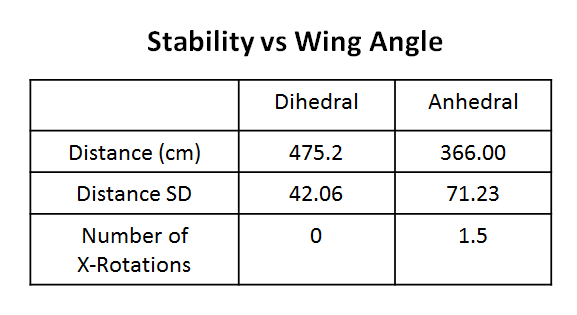
\includegraphics[scale=0.5]{figures/angles.png}
		\caption{Flight distance and stability at different wing angles.}
	\label{fig:angles}
\end{figure}

The flight was longer and more stable when the wing was dihedral. Dihedral wing produced smaller standard deviation in flight range and zero number of rotation. Furthermore, all rotations in the anhedral case occurred in x-direction, suggesting a very poor lateral stability. This result is consistent with analysis done in section~\ref{sec:dihedral}.

\subsection{Flight Distance and Stability vs Aspect Ratio}

To explore the relation between flight range/stability and aspect ratio, we constructed four models of The Arrow with different aspect ratios. We used paper of different dimensions but same area in order to control the paper airplane weight. We then launched each of them in the manner described in section~\ref{sec:arrow}, and recorded flight distance and stability data. To reduce measurement noise, we launched each paper airplane ten times and averaged the measurements. See Figure~\ref{fig:aspectratioresult} for the dimensions of each paper airplanes and the flight data. 

\begin{figure}[hl]
	\centering
		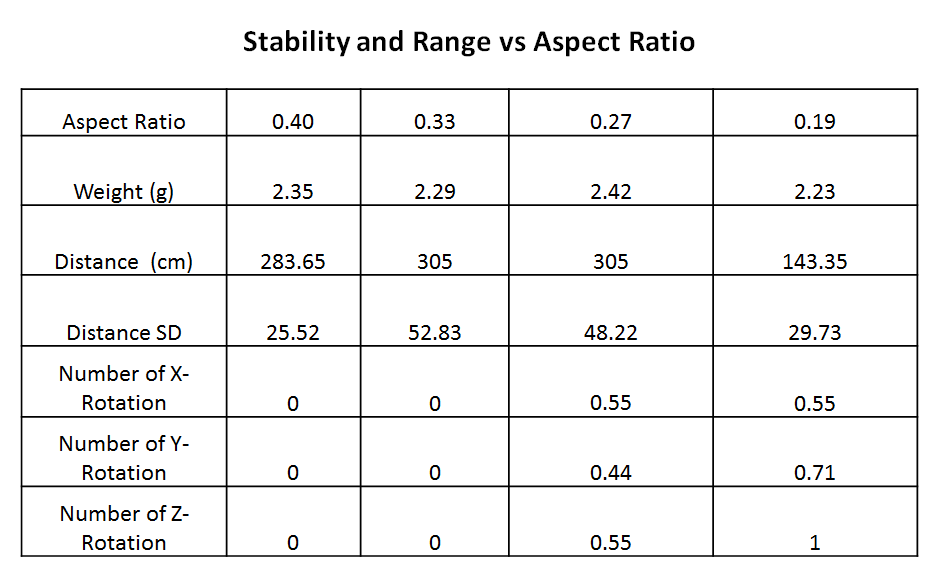
\includegraphics[scale=0.5]{figures/aspectratioresult.png}
		\caption{Flight distance and stability vs aspect ratios. As the aspect ratio decreases}
	\label{fig:aspectratioresult}
\end{figure}

As aspect ratio decreased, we observed less stable flights. When aspect ratio equaled to 0.27 and 0.19, we saw extremely turbulent flights with rotations in all directions. Flights with aspect ratio = 0.40 were more stable than flights with aspect ratio = 0.33, since they had smaller standard deviation of distance traveled. As aspect ratio increases, the lift force and air time should also increase. As a result, the paper airplane should travel longer distance. Our measurement confirmed this trend except at the case of aspect ratio = $0.4$, in which the flight distance was shorter than that from the case of aspect ration = $0.33$. We believed the difference in Reynolds number contributed to this discrepancy. At aspect ratio = 0.4, the Reynolds' number was calculated to be 
$60000$; however, at aspect ratio = 0.33, the Reynolds number was larger since the paper ariplane was longer. Laminar separtion bubbles occur on the upper surface of most airfoils at Reynolds numbers above $50000$. The bubbles become larger as the Reynolds number decreases, resulting in a rapid deterioration in performance, and substantial decrease in L/D \cite{mueller}. As a result, the flight range was smaller in the case of aspect ratio =$0.4$ compared to aspect ratio = $0.33$. 

  